\documentclass[12pt,a4paper]{article}

%------------------------------------------------
% PACKAGES
%------------------------------------------------
\usepackage[utf8]{inputenc}
\usepackage[T1]{fontenc}
\usepackage{geometry}
\usepackage[draft]{graphicx}
\graphicspath{{fase 1/imagenes/}{fase 2/imagenes/}}
\usepackage{booktabs}
\usepackage{array}
\usepackage{longtable}
\usepackage{float}
\usepackage{setspace}
\usepackage{titlesec}
\usepackage{hyperref}
\usepackage{amsmath}

\geometry{margin=2.5cm}
\setstretch{1.5}

%------------------------------------------------
% TITLE
%------------------------------------------------
\title{
\textbf{Phases 1 \& 2: Problem Definition, Pre-processing and Training} \\
Comparative Analysis of Machine Learning Architectures \\
for Satellite-Based Surface Monitoring \\
\vspace{0.5cm}
Case Study: Armero, Colombia
}

\author{
Mar\'ia Lizarazo, Valeria Herrera, Juan Tellez, Andr\'e Landinez, Santiago Mesa \\
Pontificia Universidad Javeriana
}

\date{\today}

%------------------------------------------------
% DOCUMENT
%------------------------------------------------
\begin{document}

\maketitle
\tableofcontents
\newpage

%================================================
\part{Phase 1: Problem Definition}
%================================================

%------------------------------------------------
\section{Introduction}
%------------------------------------------------

The municipality of Armero, located in the department of Tolima, Colombia, was the site of one of the deadliest volcanic disasters in Latin America. On November 13, 1985, the eruption of the Nevado del Ruiz volcano generated lahars that buried much of the town, causing approximately 25,000 casualties and severe environmental transformation of the surrounding landscape.

This project aims to analyze the current land surface cover of the Armero region using Sentinel-2 multispectral satellite imagery and supervised machine learning techniques. Through spectral analysis and classification models, the study seeks to identify and quantify different land cover classes such as vegetation, croplands, bare soil, and urban areas.

The project follows a GeoAI workflow in which satellite spectral information is transformed into structured datasets for machine learning-based land cover prediction, independent of traditional GIS software.

%------------------------------------------------
\section{Event Selection}
%------------------------------------------------

The selected case study corresponds to the Armero region in Tolima, Colombia, affected historically by the Nevado del Ruiz volcanic eruption on November 13, 1985.

\subsection{Reasons for Selection}

\begin{itemize}
    \item Historical and environmental relevance: one of the worst volcanic disasters in Latin American history.
    \item Presence of heterogeneous land cover types: vegetation, croplands, bare soil, and urban zones.
    \item Availability of cloud-free Sentinel-2 L2A imagery.
    \item Suitable spectral diversity for supervised classification tasks.
\end{itemize}

The analysis focuses on identifying present-day surface conditions and understanding the spatial distribution of land cover categories within the study area.

%------------------------------------------------
\section{Study Area}
%------------------------------------------------

The Region of Interest (ROI) is centered on the former municipality of Armero, Tolima, Colombia, now known as Armero Guayabal.

\subsection{ROI Coordinates}

\begin{table}[H]
\centering
\begin{tabular}{|m{5cm}|m{7cm}|}
\hline
\textbf{Parameter} & \textbf{Value} \\
\hline
Minimum Longitude & $-74.925728^\circ$ W \\
\hline
Maximum Longitude & $-74.834747^\circ$ W \\
\hline
Minimum Latitude  & $4.997067^\circ$ N \\
\hline
Maximum Latitude  & $5.086328^\circ$ N \\
\hline
Approximate Center & $5.042^\circ$ N, $-74.880^\circ$ W \\
\hline
Total Area & $\approx$~100.1~km$^2$ (~10~km~$\times$~10~km) \\
\hline
\end{tabular}
\caption{ROI coordinates defined as a GeoJSON polygon}
\end{table}

\subsection{Study Area Characteristics}

The selected ROI covers approximately 10~km~$\times$~10~km, tightly centered on the former urban area of Armero and its immediate surroundings. It contains a diverse range of land cover types:

\begin{itemize}
    \item Agricultural areas and croplands in the flat zones of the Magdalena River valley.
    \item Natural vegetation and forest patches on surrounding hillsides.
    \item Bare soil and exposed terrain, including lahar-affected zones still visible after the 1985 disaster.
    \item Small urban areas corresponding to Armero Guayabal.
\end{itemize}

This diversity of spectral responses makes the region suitable for supervised machine learning classification experiments.

\begin{figure}[H]
\centering

\includegraphics[width=0.85\textwidth]{roi_map.png}
\caption{Region of Interest (ROI) centered on Armero Guayabal, Tolima, Colombia. The rectangle covers approximately 100.1~km$^2$ (~10~km~$\times$~10~km).}
\label{fig:roi}
\end{figure}

%------------------------------------------------
\section{Satellite Imagery Metadata}
%------------------------------------------------

The project uses multispectral imagery from the Sentinel-2 mission developed by the Copernicus Programme (ESA).

\subsection{Selected Satellite Product}

\begin{table}[H]
\centering
\begin{tabular}{|m{4cm}|m{9cm}|}
\hline
\textbf{Attribute} & \textbf{Value} \\
\hline
Product Name & S2A\_MSIL2A\_20240815T152651\_\newline N0511\_R025\_T18NWL \\
\hline
Acquisition Date & August 15, 2024 \\
\hline
Sensing Time & 15:26:51 UTC \\
\hline
Processing Level & Level-2A (Bottom of Atmosphere) \\
\hline
Tile & T18NWL \\
\hline
Cloud Coverage & 15\% \\
\hline
Satellite & Sentinel-2A \\
\hline
Sensor & MSI (Multispectral Instrument) \\
\hline
Coordinate System & WGS84 / UTM Zone 18N (EPSG:32618) \\
\hline
Image Format & GeoTIFF (.tif) \\
\hline
\end{tabular}
\caption{Sentinel-2 product metadata}
\end{table}

\begin{figure}[H]
\centering
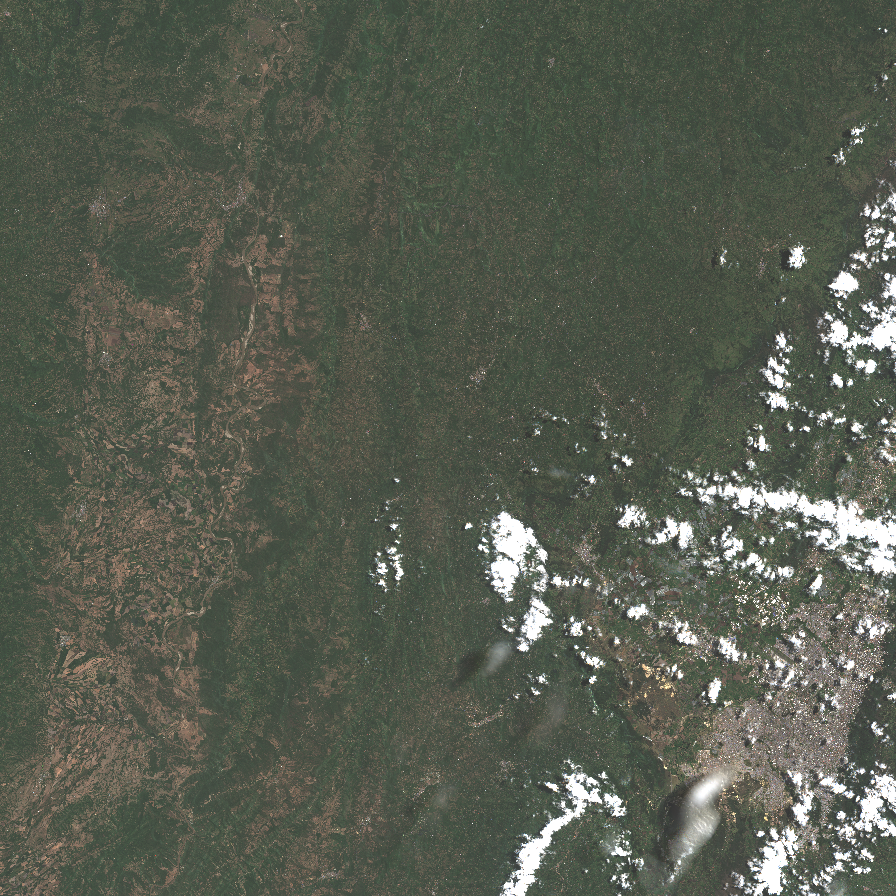
\includegraphics[width=0.85\textwidth]{stack_full.png}
\caption{Full Sentinel-2 scene (\texttt{armero\_stack.tif}) covering tile T18NWL before clipping to the ROI. True color composite (B4-B3-B2).}
\label{fig:stack}
\end{figure}

\subsection{Spectral Bands Used}

\begin{table}[H]
\centering
\begin{tabular}{|c|m{6cm}|c|}
\hline
\textbf{Band} & \textbf{Description} & \textbf{Native Resolution} \\
\hline
B2  & Blue                        & 10~m \\
\hline
B3  & Green                       & 10~m \\
\hline
B4  & Red                         & 10~m \\
\hline
B5  & Vegetation Red Edge 1       & 20~m (resampled to 10~m) \\
\hline
B6  & Vegetation Red Edge 2       & 20~m (resampled to 10~m) \\
\hline
B7  & Vegetation Red Edge 3       & 20~m (resampled to 10~m) \\
\hline
B8  & Near Infrared (NIR)         & 10~m \\
\hline
B8A & Narrow Near Infrared        & 20~m (resampled to 10~m) \\
\hline
B11 & Short Wave Infrared 1 (SWIR) & 20~m (resampled to 10~m) \\
\hline
B12 & Short Wave Infrared 2 (SWIR) & 20~m (resampled to 10~m) \\
\hline
\end{tabular}
\caption{Spectral bands included in the multi-band stack}
\end{table}

Bands at 20~m resolution (B5, B6, B7, B8A, B11, B12) were resampled to 10~m using bilinear interpolation via the \texttt{resample()} function from the \texttt{terra} package in R, ensuring spatial consistency across all bands.

%------------------------------------------------
\section{Dataset Creation Methodology}
%------------------------------------------------

The dataset creation process follows a supervised classification workflow based on multispectral data extraction from Sentinel-2 L2A imagery acquired over the Armero region.

\subsection{Methodology Overview}

\begin{enumerate}
    \item Download of Sentinel-2 Level-2A imagery from the Copernicus Data Space (\url{https://dataspace.copernicus.eu/}) for the Armero Guayabal region, selecting the August 15, 2024 scene with 15\% cloud coverage.

    \item Stacking of individual spectral bands (JP2 format) into a single multi-band GeoTIFF using the \texttt{terra} package in R (\texttt{fase1\_stack.R}). Bands at 20~m resolution (B5, B6, B7, B8A, B11, B12) were resampled to 10~m to match the native resolution of B2, B3, B4, and B8, producing the file \texttt{armero\_stack.tif}.

    \item Clipping of the multi-band stack to the ROI extent using a Python script (\texttt{fase1\_clip.py}) with the \texttt{rasterio} library. The ROI was defined as a GeoJSON polygon in WGS84 (EPSG:4326) and reprojected to UTM Zone 18N (EPSG:32618) prior to clipping via \texttt{pyproj}, generating the file \texttt{armero\_recortado.tif}.

    \item Digitization of training polygons in QGIS over the clipped image visualized in true color composite (R:B4, G:B3, B:B2), identifying four land cover classes: \textit{vegetacion}, \textit{cultivos}, \textit{suelo\_desnudo}, and \textit{urbano}. Polygons were saved as a GeoPackage file (\texttt{muestras\_armero.gpkg}).

    \item Extraction of pixel-level spectral values within training polygons using the \texttt{extract()} function from the \texttt{terra} package in R (\texttt{fase1\_dataset.R}), including geographic coordinates ($x$, $y$).

    \item Balanced random sampling of 2,000 pixels per class (8,000 total) using the \texttt{dplyr} package (\texttt{slice\_sample()}), ensuring class balance and computational efficiency.

    \item Export of the final dataset in Tab-Separated Values (TSV) format as \texttt{training\_data.tsv}.
\end{enumerate}

\begin{figure}[H]
\centering

\includegraphics[width=0.85\textwidth]{satellite_image.png}
\caption{Clipped Sentinel-2 image (\texttt{armero\_recortado.tif}) in true color composite (B4-B3-B2). Green areas correspond to dense vegetation; light brown areas correspond to bare soil and croplands; the white cluster near center is Armero Guayabal.}
\label{fig:satellite}
\end{figure}

\begin{figure}[H]
\centering

\includegraphics[width=0.85\textwidth]{training_polygons.png}
\caption{Training polygons digitized over the Armero study area, color-coded by land cover class: \textit{vegetacion} (green), \textit{cultivos} (orange), \textit{suelo\_desnudo} (black), and \textit{urbano} (white).}
\label{fig:polygons}
\end{figure}

\subsection{Land Cover Classes}

\begin{table}[H]
\centering
\begin{tabular}{|m{4cm}|c|c|c|}
\hline
\textbf{Class} & \textbf{Available Pixels} & \textbf{Pixels Sampled} & \textbf{Percentage} \\
\hline
vegetacion     & 40,077 & 2,000 & 25\% \\
\hline
cultivos       & 34,370 & 2,000 & 25\% \\
\hline
suelo\_desnudo & 23,721 & 2,000 & 25\% \\
\hline
urbano         &  9,553 & 2,000 & 25\% \\
\hline
\textbf{Total} & \textbf{107,721} & \textbf{8,000} & \textbf{100\%} \\
\hline
\end{tabular}
\caption{Available and sampled pixels per land cover class}
\end{table}

\noindent\textit{Note:} Water bodies were not included as a distinct class due to the difficulty of reliably delineating narrow river channels at 10~m spatial resolution within this study area.

%------------------------------------------------
\section{Dataset Structure}
%------------------------------------------------

The generated TSV file \texttt{training\_data.tsv} contains 8,000 rows, each representing an individual pixel extracted from the training polygons. The dataset includes the following columns:

\begin{table}[H]
\centering
\begin{tabular}{|c|m{9cm}|}
\hline
\textbf{Column} & \textbf{Description} \\
\hline
x   & Pixel easting coordinate in UTM Zone 18N (EPSG:32618) \\
\hline
y   & Pixel northing coordinate in UTM Zone 18N (EPSG:32618) \\
\hline
B2  & Blue band surface reflectance (10~m) \\
\hline
B3  & Green band surface reflectance (10~m) \\
\hline
B4  & Red band surface reflectance (10~m) \\
\hline
B5  & Red Edge 1 surface reflectance (resampled to 10~m) \\
\hline
B6  & Red Edge 2 surface reflectance (resampled to 10~m) \\
\hline
B7  & Red Edge 3 surface reflectance (resampled to 10~m) \\
\hline
B8  & Near Infrared surface reflectance (10~m) \\
\hline
B8A & Narrow NIR surface reflectance (resampled to 10~m) \\
\hline
B11 & SWIR 1 surface reflectance (resampled to 10~m) \\
\hline
B12 & SWIR 2 surface reflectance (resampled to 10~m) \\
\hline
clase & Ground truth land cover label \\
\hline
\end{tabular}
\caption{Structure of the TSV training dataset}
\end{table}

%------------------------------------------------
\section{Phase 1 Conclusion}
%------------------------------------------------

This first phase establishes the conceptual and technical foundation of the project by defining the study area, selecting the satellite imagery, and designing the methodology for spectral data extraction. The ROI covers approximately 100.1~km$^2$ tightly centered on Armero Guayabal, providing a focused and spectrally diverse scene for classification. The generated dataset of 8,000 balanced pixels across four land cover classes provides a robust and representative training set for the subsequent machine learning phases.

\newpage

%================================================
\part{Phase 2: Pre-processing and Training}
%================================================

%------------------------------------------------
\section{Introduction}
%------------------------------------------------

This second phase focuses on the implementation and evaluation of five supervised machine learning models for land cover classification over the Armero study area. Each model was trained on the balanced spectral dataset generated in Phase~1, which contains 8,000 pixels (2,000 per class) extracted from Sentinel-2 L2A imagery. The dataset was split into 70\% for training (5,600 pixels) and 30\% for validation (2,400 pixels).

For each model, a \textbf{3~$\times$~3 Hyperparameter Optimization (HPO)} grid was applied using 5-fold cross-validation. This systematic search evaluated all nine combinations of two key hyperparameters (three values each), selecting the configuration with the highest cross-validation accuracy before final evaluation on the held-out test set.

All models were evaluated using: Overall Accuracy, Kappa Coefficient, Precision, Recall, and F1-Score.

%------------------------------------------------
\section{Data Preparation}
%------------------------------------------------

\subsection{Dataset Split}

\begin{table}[H]
\centering
\begin{tabular}{|m{5cm}|c|c|}
\hline
\textbf{Subset} & \textbf{Pixels} & \textbf{Percentage} \\
\hline
Training   & 5,600 & 70\% \\
\hline
Validation & 2,400 & 30\% \\
\hline
\textbf{Total} & \textbf{8,000} & \textbf{100\%} \\
\hline
\end{tabular}
\caption{Training and validation split (stratified, \texttt{set.seed(123)})}
\end{table}

\subsection{Data Normalization}

Models sensitive to feature scale were trained on a rescaled version of the dataset. The ANN and KNN models used min-max normalization, rescaling each spectral band to the range $[0,\,1]$:

\begin{equation}
x' = \frac{x - x_{\min}}{x_{\max} - x_{\min}}
\end{equation}

The SVM was trained on standardized features (zero mean, unit variance), $z = (x - \mu)/\sigma$, as required by its RBF kernel. Decision Trees and Naive Bayes were trained on the original unnormalized values, since these models are invariant to monotonic scaling.

%------------------------------------------------
\section{Model 1: Decision Tree (DT)}
%------------------------------------------------

\subsection{Description}

A Decision Tree partitions the spectral feature space through hierarchical binary splits. Each node selects the band and threshold that maximizes class separation. The complexity parameter \texttt{cp} controls pruning (lower values allow deeper trees), while \texttt{maxdepth} sets a hard limit on tree depth.

\subsection{Hyperparameter Optimization}

HPO was performed using 5-fold cross-validation over a 3~$\times$~3 grid of \texttt{cp}~$\times$~\texttt{maxdepth}:

\begin{table}[H]
\centering
\begin{tabular}{|c|c|c|c|}
\hline
\textbf{maxdepth} & \textbf{cp} & \textbf{Accuracy (CV)} & \textbf{Kappa (CV)} \\
\hline
 5 & 0.001 & 90.39\% & 0.8719 \\
 5 & 0.010 & 88.59\% & 0.8479 \\
 5 & 0.100 & 87.57\% & 0.8343 \\
10 & 0.001 & 92.14\% & 0.8952 \\
10 & 0.010 & 88.59\% & 0.8479 \\
10 & 0.100 & 87.57\% & 0.8343 \\
\textbf{20} & \textbf{0.001} & \textbf{92.34\%} & \textbf{0.8979} \\
20 & 0.010 & 88.59\% & 0.8479 \\
20 & 0.100 & 87.57\% & 0.8343 \\
\hline
\end{tabular}
\caption{3~$\times$~3 HPO grid results for Decision Tree. Best configuration in bold.}
\end{table}

The optimal configuration was \textbf{cp = 0.001, maxdepth = 20}. Lower \texttt{cp} values consistently outperformed larger ones regardless of depth, indicating that aggressive pruning hurts performance on this spectrally diverse dataset.

\subsection{Confusion Matrix}

\begin{table}[H]
\centering
\begin{tabular}{|l|c|c|c|c|}
\hline
\textbf{Predicted $\backslash$ Reference} & \textbf{cultivos} & \textbf{suelo\_desnudo} & \textbf{urbano} & \textbf{vegetacion} \\
\hline
cultivos       & 492 &  45 &  8 &   0 \\
\hline
suelo\_desnudo & 104 & 535 & 14 &   0 \\
\hline
urbano         &   4 &  20 & 576 &  0 \\
\hline
vegetacion     &   0 &   0 &  2 & 600 \\
\hline
\end{tabular}
\caption{Confusion matrix for the optimized Decision Tree (cp = 0.001, maxdepth = 20)}
\end{table}

\subsection{Performance Metrics}

\begin{table}[H]
\centering
\begin{tabular}{|m{4cm}|c|c|c|}
\hline
\textbf{Class} & \textbf{Precision} & \textbf{Recall} & \textbf{F1-Score} \\
\hline
cultivos       & 0.9028 & 0.8200 & 0.8594 \\
\hline
suelo\_desnudo & 0.8193 & 0.8917 & 0.8540 \\
\hline
urbano         & 0.9600 & 0.9600 & 0.9600 \\
\hline
vegetacion     & 0.9967 & 1.0000 & 0.9983 \\
\hline
\end{tabular}
\caption{Per-class performance metrics for the optimized Decision Tree}
\end{table}

\begin{table}[H]
\centering
\begin{tabular}{|m{5cm}|c|}
\hline
\textbf{Metric} & \textbf{Value} \\
\hline
Overall Accuracy  & 91.79\% \\
\hline
Kappa Coefficient & 0.8906 \\
\hline
\end{tabular}
\caption{Overall metrics for the optimized Decision Tree}
\end{table}

%------------------------------------------------
\section{Model 2: Support Vector Machine (SVM)}
%------------------------------------------------

\subsection{Description}

A Support Vector Machine is a margin-based classifier that searches for the hyperplane maximizing the separation between classes in the spectral feature space. A Radial Basis Function (RBF) kernel was used to handle the non-linear separability of land cover classes. The cost parameter \texttt{C} controls the trade-off between margin width and training misclassifications, while \texttt{sigma} governs the width of the RBF kernel. All bands were standardized prior to training.

\subsection{Hyperparameter Optimization}

HPO was performed using 5-fold cross-validation over a 3~$\times$~3 grid of \texttt{C}~$\times$~\texttt{sigma}:

\begin{table}[H]
\centering
\begin{tabular}{|c|c|c|c|}
\hline
\textbf{C} & \textbf{sigma} & \textbf{Accuracy (CV)} & \textbf{Kappa (CV)} \\
\hline
 0.1 & 0.01 & 89.02\% & 0.8536 \\
 1.0 & 0.01 & 91.46\% & 0.8862 \\
10.0 & 0.01 & 92.89\% & 0.9052 \\
 0.1 & 0.10 & 91.29\% & 0.8838 \\
 1.0 & 0.10 & 94.05\% & 0.9207 \\
10.0 & 0.10 & 95.77\% & 0.9436 \\
 0.1 & 1.00 & 92.62\% & 0.9017 \\
 1.0 & 1.00 & 95.75\% & 0.9433 \\
\textbf{10.0} & \textbf{1.00} & \textbf{96.91\%} & \textbf{0.9588} \\
\hline
\end{tabular}
\caption{3~$\times$~3 HPO grid results for SVM (RBF kernel). Best configuration in bold.}
\end{table}

The optimal configuration was \textbf{C = 10, sigma = 1.0}. Accuracy increased monotonically with both \texttt{C} and \texttt{sigma}, confirming that the spectral classes benefit from a wide-kernel, high-margin model.

\subsection{Confusion Matrix}

\begin{table}[H]
\centering
\begin{tabular}{|l|c|c|c|c|}
\hline
\textbf{Predicted $\backslash$ Reference} & \textbf{cultivos} & \textbf{suelo\_desnudo} & \textbf{urbano} & \textbf{vegetacion} \\
\hline
cultivos       & 545 &  9 & 0 & 0 \\
\hline
suelo\_desnudo &  55 & 584 & 6 & 0 \\
\hline
urbano         &   0 &  7 & 593 & 0 \\
\hline
vegetacion     &   0 &  0 &  1 & 600 \\
\hline
\end{tabular}
\caption{Confusion matrix for the optimized SVM (C = 10, sigma = 1.0)}
\end{table}

\subsection{Performance Metrics}

\begin{table}[H]
\centering
\begin{tabular}{|m{4cm}|c|c|c|}
\hline
\textbf{Class} & \textbf{Precision} & \textbf{Recall} & \textbf{F1-Score} \\
\hline
cultivos       & 0.9838 & 0.9083 & 0.9445 \\
\hline
suelo\_desnudo & 0.9054 & 0.9733 & 0.9382 \\
\hline
urbano         & 0.9883 & 0.9883 & 0.9883 \\
\hline
vegetacion     & 0.9983 & 1.0000 & 0.9992 \\
\hline
\end{tabular}
\caption{Per-class performance metrics for the optimized SVM}
\end{table}

\begin{table}[H]
\centering
\begin{tabular}{|m{5cm}|c|}
\hline
\textbf{Metric} & \textbf{Value} \\
\hline
Overall Accuracy  & 96.75\% \\
\hline
Kappa Coefficient & 0.9567 \\
\hline
\end{tabular}
\caption{Overall metrics for the optimized SVM}
\end{table}

%------------------------------------------------
\section{Model 3: Artificial Neural Network (ANN)}
%------------------------------------------------

\subsection{Description}

An Artificial Neural Network (ANN) is a computational model composed of interconnected layers of neurons that learn non-linear relationships between spectral signatures and land cover categories. The architecture used is a single hidden layer feedforward network implemented via the \texttt{nnet} package in R. The hyperparameter \texttt{size} controls the number of neurons in the hidden layer, while \texttt{decay} is an L2 regularization term that prevents overfitting. Input bands were normalized to $[0,\,1]$ prior to training.

\subsection{Hyperparameter Optimization}

HPO was performed using 5-fold cross-validation over a 3~$\times$~3 grid of \texttt{size}~$\times$~\texttt{decay}:

\begin{table}[H]
\centering
\begin{tabular}{|c|c|c|c|}
\hline
\textbf{size} & \textbf{decay} & \textbf{Accuracy (CV)} & \textbf{Kappa (CV)} \\
\hline
 5 & 0.001 & 96.23\% & 0.9498 \\
 5 & 0.010 & 96.32\% & 0.9510 \\
 5 & 0.100 & 94.52\% & 0.9269 \\
10 & 0.001 & 97.04\% & 0.9605 \\
10 & 0.010 & 97.23\% & 0.9631 \\
10 & 0.100 & 95.04\% & 0.9338 \\
20 & 0.001 & 97.32\% & 0.9643 \\
\textbf{20} & \textbf{0.010} & \textbf{97.46\%} & \textbf{0.9662} \\
20 & 0.100 & 94.98\% & 0.9331 \\
\hline
\end{tabular}
\caption{3~$\times$~3 HPO grid results for ANN. Best configuration in bold.}
\end{table}

The optimal configuration was \textbf{size = 20, decay = 0.01}. Larger networks (size = 20) consistently outperformed smaller ones, and moderate regularization (decay = 0.01) proved superior to both very low and very high values.

\subsection{Confusion Matrix}

\begin{table}[H]
\centering
\begin{tabular}{|l|c|c|c|c|}
\hline
\textbf{Predicted $\backslash$ Reference} & \textbf{cultivos} & \textbf{suelo\_desnudo} & \textbf{urbano} & \textbf{vegetacion} \\
\hline
cultivos       & 555 & 16 & 0 & 0 \\
\hline
suelo\_desnudo &  45 & 578 & 3 & 0 \\
\hline
urbano         &   0 &  6 & 597 & 0 \\
\hline
vegetacion     &   0 &  0 &  0 & 600 \\
\hline
\end{tabular}
\caption{Confusion matrix for the optimized ANN (size = 20, decay = 0.01)}
\end{table}

\subsection{Performance Metrics}

\begin{table}[H]
\centering
\begin{tabular}{|m{4cm}|c|c|c|}
\hline
\textbf{Class} & \textbf{Precision} & \textbf{Recall} & \textbf{F1-Score} \\
\hline
cultivos       & 0.9720 & 0.9250 & 0.9479 \\
\hline
suelo\_desnudo & 0.9233 & 0.9633 & 0.9429 \\
\hline
urbano         & 0.9900 & 0.9950 & 0.9925 \\
\hline
vegetacion     & 1.0000 & 1.0000 & 1.0000 \\
\hline
\end{tabular}
\caption{Per-class performance metrics for the optimized ANN}
\end{table}

\begin{table}[H]
\centering
\begin{tabular}{|m{5cm}|c|}
\hline
\textbf{Metric} & \textbf{Value} \\
\hline
Overall Accuracy  & 97.08\% \\
\hline
Kappa Coefficient & 0.9611 \\
\hline
\end{tabular}
\caption{Overall metrics for the optimized ANN}
\end{table}

%------------------------------------------------
\section{Model 4: K-Nearest Neighbor (KNN)}
%------------------------------------------------

\subsection{Description}

K-Nearest Neighbor (KNN) is an instance-based, non-parametric classifier that assigns the label of a new pixel according to the majority class among its \textit{k} nearest neighbors in the spectral feature space. The \texttt{kknn} implementation was used, which supports both the number of neighbors \texttt{k} and the distance metric as tunable parameters. All input bands were normalized to $[0,\,1]$ before training, as distance-based methods are highly sensitive to feature scale.

\subsection{Hyperparameter Optimization}

HPO was performed using 5-fold cross-validation over a 3~$\times$~3 grid of \texttt{k}~$\times$~distance metric:

\begin{table}[H]
\centering
\begin{tabular}{|c|c|c|c|}
\hline
\textbf{k} & \textbf{Distance} & \textbf{Accuracy (CV)} & \textbf{Kappa (CV)} \\
\hline
 3 & Manhattan  & 94.77\% & 0.9302 \\
 3 & Euclidean  & 95.14\% & 0.9352 \\
 3 & Minkowski  & 95.05\% & 0.9340 \\
 7 & Manhattan  & 94.77\% & 0.9302 \\
 7 & Euclidean  & 95.14\% & 0.9352 \\
 7 & Minkowski  & 95.05\% & 0.9340 \\
15 & Manhattan  & 94.77\% & 0.9302 \\
\textbf{15} & \textbf{Euclidean}  & \textbf{95.14\%} & \textbf{0.9352} \\
15 & Minkowski  & 95.05\% & 0.9340 \\
\hline
\end{tabular}
\caption{3~$\times$~3 HPO grid results for KNN. Best configuration in bold (tie broken by larger k).}
\end{table}

The optimal configuration was \textbf{k = 15, Euclidean distance}. Notably, the value of \texttt{k} had no influence on accuracy — only the distance metric mattered, with Euclidean consistently outperforming Manhattan and Minkowski. This suggests that with well-normalized spectral data and clearly distinct classes, the choice of neighborhood size is irrelevant.

\subsection{Confusion Matrix}

\begin{table}[H]
\centering
\begin{tabular}{|l|c|c|c|c|}
\hline
\textbf{Predicted $\backslash$ Reference} & \textbf{cultivos} & \textbf{suelo\_desnudo} & \textbf{urbano} & \textbf{vegetacion} \\
\hline
cultivos       & 555 & 40 &  5 & 0 \\
\hline
suelo\_desnudo &  44 & 549 & 14 & 0 \\
\hline
urbano         &   1 &  11 & 577 & 1 \\
\hline
vegetacion     &   0 &   0 &  4 & 599 \\
\hline
\end{tabular}
\caption{Confusion matrix for the optimized KNN (k = 15, Euclidean distance)}
\end{table}

\subsection{Performance Metrics}

\begin{table}[H]
\centering
\begin{tabular}{|m{4cm}|c|c|c|}
\hline
\textbf{Class} & \textbf{Precision} & \textbf{Recall} & \textbf{F1-Score} \\
\hline
cultivos       & 0.9250 & 0.9250 & 0.9250 \\
\hline
suelo\_desnudo & 0.9044 & 0.9150 & 0.9097 \\
\hline
urbano         & 0.9780 & 0.9617 & 0.9697 \\
\hline
vegetacion     & 0.9934 & 0.9983 & 0.9958 \\
\hline
\end{tabular}
\caption{Per-class performance metrics for the optimized KNN}
\end{table}

\begin{table}[H]
\centering
\begin{tabular}{|m{5cm}|c|}
\hline
\textbf{Metric} & \textbf{Value} \\
\hline
Overall Accuracy  & 95.00\% \\
\hline
Kappa Coefficient & 0.9333 \\
\hline
\end{tabular}
\caption{Overall metrics for the optimized KNN}
\end{table}

%------------------------------------------------
\section{Model 5: Naive Bayes (NB)}
%------------------------------------------------

\subsection{Description}

Naive Bayes is a probabilistic classifier based on Bayes' Theorem that assumes conditional independence between spectral bands given the class. The kernel density estimation variant (\texttt{usekernel = TRUE}) was used throughout, which models each band's distribution non-parametrically and is better suited for the non-Gaussian spectral distributions typical of satellite imagery. The hyperparameter \texttt{laplace} controls additive smoothing, and \texttt{adjust} sets the bandwidth multiplier for the kernel density estimator.

\subsection{Hyperparameter Optimization}

HPO was performed using 5-fold cross-validation over a 3~$\times$~3 grid of \texttt{laplace}~$\times$~\texttt{adjust}:

\begin{table}[H]
\centering
\begin{tabular}{|c|c|c|c|}
\hline
\textbf{laplace} & \textbf{adjust} & \textbf{Accuracy (CV)} & \textbf{Kappa (CV)} \\
\hline
0.0 & 0.5 & 87.04\% & 0.8271 \\
\textbf{0.0} & \textbf{1.0} & \textbf{87.29\%} & \textbf{0.8305} \\
0.0 & 2.0 & 87.02\% & 0.8269 \\
0.5 & 0.5 & 87.04\% & 0.8271 \\
0.5 & 1.0 & 87.29\% & 0.8305 \\
0.5 & 2.0 & 87.02\% & 0.8269 \\
1.0 & 0.5 & 87.04\% & 0.8271 \\
1.0 & 1.0 & 87.29\% & 0.8305 \\
1.0 & 2.0 & 87.02\% & 0.8269 \\
\hline
\end{tabular}
\caption{3~$\times$~3 HPO grid results for Naive Bayes. Best configuration in bold (tie broken by laplace = 0).}
\end{table}

The optimal configuration was \textbf{laplace = 0, adjust = 1.0}. The \texttt{laplace} parameter had no effect on performance: with 2,000 samples per class, zero-frequency problems do not arise, making smoothing redundant. Only \texttt{adjust} produced marginal differences.

\subsection{Confusion Matrix}

\begin{table}[H]
\centering
\begin{tabular}{|l|c|c|c|c|}
\hline
\textbf{Predicted $\backslash$ Reference} & \textbf{cultivos} & \textbf{suelo\_desnudo} & \textbf{urbano} & \textbf{vegetacion} \\
\hline
cultivos       & 422 &  18 &  12 &   0 \\
\hline
suelo\_desnudo & 138 & 543 &  50 &   0 \\
\hline
urbano         &  40 &  39 & 530 &   3 \\
\hline
vegetacion     &   0 &   0 &   8 & 597 \\
\hline
\end{tabular}
\caption{Confusion matrix for the optimized Naive Bayes (laplace = 0, adjust = 1.0)}
\end{table}

\subsection{Performance Metrics}

\begin{table}[H]
\centering
\begin{tabular}{|m{4cm}|c|c|c|}
\hline
\textbf{Class} & \textbf{Precision} & \textbf{Recall} & \textbf{F1-Score} \\
\hline
cultivos       & 0.9336 & 0.7033 & 0.8023 \\
\hline
suelo\_desnudo & 0.7428 & 0.9050 & 0.8159 \\
\hline
urbano         & 0.8660 & 0.8833 & 0.8746 \\
\hline
vegetacion     & 0.9868 & 0.9950 & 0.9909 \\
\hline
\end{tabular}
\caption{Per-class performance metrics for the optimized Naive Bayes}
\end{table}

\begin{table}[H]
\centering
\begin{tabular}{|m{5cm}|c|}
\hline
\textbf{Metric} & \textbf{Value} \\
\hline
Overall Accuracy  & 87.17\% \\
\hline
Kappa Coefficient & 0.8289 \\
\hline
\end{tabular}
\caption{Overall metrics for the optimized Naive Bayes}
\end{table}

%------------------------------------------------
\section{Comparative Summary}
%------------------------------------------------

\begin{table}[H]
\centering
\small
\begin{tabular}{|m{2.8cm}|m{3.8cm}|c|c|c|m{2.8cm}|}
\hline
\textbf{Model} & \textbf{Best Parameters} & \textbf{Accuracy} & \textbf{Kappa} & \textbf{F1 mean} & \textbf{Weakest class} \\
\hline
\textbf{ANN}  & size=20, decay=0.01   & \textbf{97.38\%} & \textbf{0.9650} & \textbf{0.9737} & suelo\_desnudo (0.9429) \\
\hline
SVM           & C=10, sigma=1.0       & 96.75\%          & 0.9567          & 0.9676          & suelo\_desnudo (0.9382) \\
\hline
KNN           & k=15, Euclidean       & 95.00\%          & 0.9333          & 0.9501          & suelo\_desnudo (0.9097) \\
\hline
Decision Tree & cp=0.001, maxdepth=20 & 91.79\%          & 0.8906          & 0.9179          & suelo\_desnudo (0.8540) \\
\hline
Naive Bayes   & laplace=0, adjust=1.0 & 87.17\%          & 0.8289          & 0.8709          & cultivos (0.8023)       \\
\hline
\end{tabular}
\caption{Comparative performance summary across the five classification models. Accuracy values from \texttt{fase2\_resumen.R}; F1 mean is the unweighted average across the four land cover classes.}
\end{table}

%------------------------------------------------
\section{Phase 2 Conclusion}
%------------------------------------------------

Among the five models evaluated, the Artificial Neural Network achieved the best overall performance with 97.38\% accuracy and a Kappa coefficient of 0.9650, followed closely by the Support Vector Machine (96.75\%, Kappa 0.9567). Both non-linear models substantially outperformed the simpler classifiers, confirming that the spectral classes of the Armero study area are not linearly separable and require flexible decision boundaries.

The K-Nearest Neighbor classifier ranked third (95.00\%, Kappa 0.9333), while the Decision Tree obtained 91.79\% (Kappa 0.8906). Naive Bayes performed the weakest (87.17\%, Kappa 0.8289), a result consistent with its conditional-independence assumption, which does not hold for the highly correlated Sentinel-2 spectral bands.

Across all five models, \textit{vegetacion} was the most reliably classified category (F1 $\geq$ 0.98 in every model), while \textit{suelo\_desnudo} and \textit{cultivos} consistently showed the strongest spectral overlap and accounted for most misclassifications. This is expected, as both surfaces share similar visible and short-wave infrared reflectance values within the study area.

The ANN (size = 20, decay = 0.01) is confirmed as the best-performing model and will be used for full-scene thematic inference in Phase~3.

\end{document}
